\documentclass{article}

\usepackage[utf8]{inputenc}

\usepackage{graphicx}

\graphicspath{ {imagens/} }
\title{Aulas de MPS}
\author{cotrim149 }
\date{March 2014}

\begin{document}

\maketitle

\section{Artigo - Defining Short and Usable Processes}

\subsection{Problemas comumente encontrados na documnetação de processos}

\begin{enumerate}
	\item Muito grande: Todo documento deve ser curto, conciso e útil.
	\item Não existem figuras: Boas documentações de processo possuem uma mistura de textos, figuras e diagramas. 
	\item Documentos com pobre "design"
	\item Inutilizável e tamanho único: A documentação não é considerada para ser utilizada pelo cliente e o processo ainda está na mente dos usuários. Muitas destas documnetações não considera o nível de entedimento de seu usuário.
	\item Tipos de informações misturadas: Informações sobre política de empresa, treinamento, padrões, processos e entre outros estão misturados no mesmo parágrafo. 
	\item Escrito sequencialmente: A documentação do processo não é para ser escrita como uma novela, logo não existe a necessidade de se ler linearmente. Um documento deste tipo é para ser usado de forma não linear. "This is why labeling is critical so that users can find information quickly"
	\item Dificil de se encontrar uma informação rapidamente: Uma documentação para processos deve ser usada para se encontrar alguma informação rapidamente. Caso não seja encontrado rapidamente, muitas vezes é feita a desistência de se usar a documentação.
	\item  Shelfware: Most process documentation becomes shelfware (i.e.collects dust on a shelf). Online processes (e.g. on an intranet) must be well designed or they will also become unused Web-ware.
 
\end{enumerate}

\subsection{Modo de documentação}
\begin{enumerate}
	\item Expert: Curto e conciso. Normalmente não inclui algum material de treinamento.
	\item Intermediario: Providencia um guia rápido mostrando as lições já aprendidas. Muito útil para pessoas que não seguem um processo ou procedimento frequentemente. Tipicamente guias e lições aprendidas não são auditáveis
	\item Iniciante: Manuais e materias de treinamento são adicionados a este material. Também é usado o material Expert e intermediario para o iniciante. 
\end{enumerate}

\subsection{O que é um bom processo?}
\paragraph{Um bom processo}, consiste em informar o passo-a-passo e como executá-lo e isso pode acontecer em 3 formas:

\begin{enumerate}
	\item Checklists
		
	\item Formulários
	\item Tabelas de passo/ação
\end{enumerate}


\section{Visão geral}
\subsection{O que é processo?}
	\paragraph{Entradas}	
	
	\begin{itemize}
	\item Atividades
	\item Papéis
	\item Políticas
	\item Ferramentas
	\item Métodos
	\end{itemize}
	\paragraph{Saidas}

	\paragraph{Processos: Processos são uma interface estável entre pessoas e tecnologias}

\subsection{Melhoria de processos de Software}
\subsubsection{Definição}
\paragraph{Diz respeito ao esforço empreendido com o objetivo de melhorar o modo como o software é desenvolvido}	
\paragraph{Melhorar a forma como o software é desenvolvido}

\subsubsection{Processos Maduro}
	\begin{itemize}
	\item Processo é um ativo de empresa
	\item A dorma de realizar o trabalho é bem definida
	\item É continuamente monitorado, documentado, e melhorado
	\item Colaboradores qualificados realizam qauisquer tarefas
	\item Qualidade do produto é obtida por meio da qualidade do proecesso	
	\end{itemize}

\subsection{Implanatção de MPS}
Diz respeito aos passos ou à estrategia adotaad melhoroa de processos de software em uma organização
Deve ser definido considerando as caracteristicas da empresa e os objetivos de melhoria	

\paragraph{Principais fases}
	\begin{enumerate}
	\item Iniciação
	\item Diagnóstico
	\item Estabelecimento/ Planejamento
	\item Ação
	\item Aprendizado	
	\end{enumerate}

\subsection{Exercícios}

\section{MPS.BR} 
\subsection{Introdução} \date{26 de Março de 2014}


\subsubsection{Softex} 
	\begin{itemize}
	\item Capacitação e inovação
	\item Mercado
	\item Qualidade e competitividade
	\end{itemize}
	
\subsubsection{Nivel CMMI}
	
\begin{center}

\begin{tabular}{|c|c|}
\hline 
Nivel & Maturidade \\ 
\hline 
Nível 5 & + \\ 
\hline 
Nível 0 & - \\ 
\hline 
\end{tabular} 

\end{center}

	
\subsubsection{O que é o MPS?} 
	
	\begin{enumerate}		
	
	\item Pequenas e médias empresas em foco a um custo acessível
	\item Modelo que esteja em conformidade com normas e padrões internacionais
	\item Definir um modelo de avaliação mais flexivel com a relidade brasileira
	
	\item Apoio 
		\begin{enumerate}
		\item MCT
		\item Financiadora de estudos e projetos
		\item SEBRAE
		\item BID		
		\end{enumerate}

\begin{center}
	\begin{tabular}{|c|c|}
	\hline 
	Níveis CMMI & Níveis MPS.BR \\
	\hline
	5 &  A\\
	\hline
	4 & B\\
	\hline
	3 & C\\
	& D\\
	& E\\
	\hline
	2 & F\\
	& G	\\
	\hline
	\end{tabular}
\end{center}
		
	\end{enumerate}
			
\subsubsection{Histórico}
	\begin{itemize}
	\item Guia Geral
	\item Guia Geral de Serviços
	\item Guia de Aquisição
	\item Guia de Avaliação
	\end{itemize}		
	

\subsubsection{Organização}
	\begin{itemize}
	\item Coordenação do programa MPS.BR(Softex)
		\begin{itemize}
		\item Equipe técnica do Modelo(ETM): Responsável por evoluções dos guias
		\item Fórum de Credenciamento e controle(FCC): Responsável por garantir que as empresas e profissionais que estão no contexto estejam credenciadas [Instituições Avaliadoras(IA)]e[Instituição Implementadoras(II)]
		
		\end{itemize}			
	\end{itemize}


\subsubsection{Modelo de Negócio}
	\begin{center}
		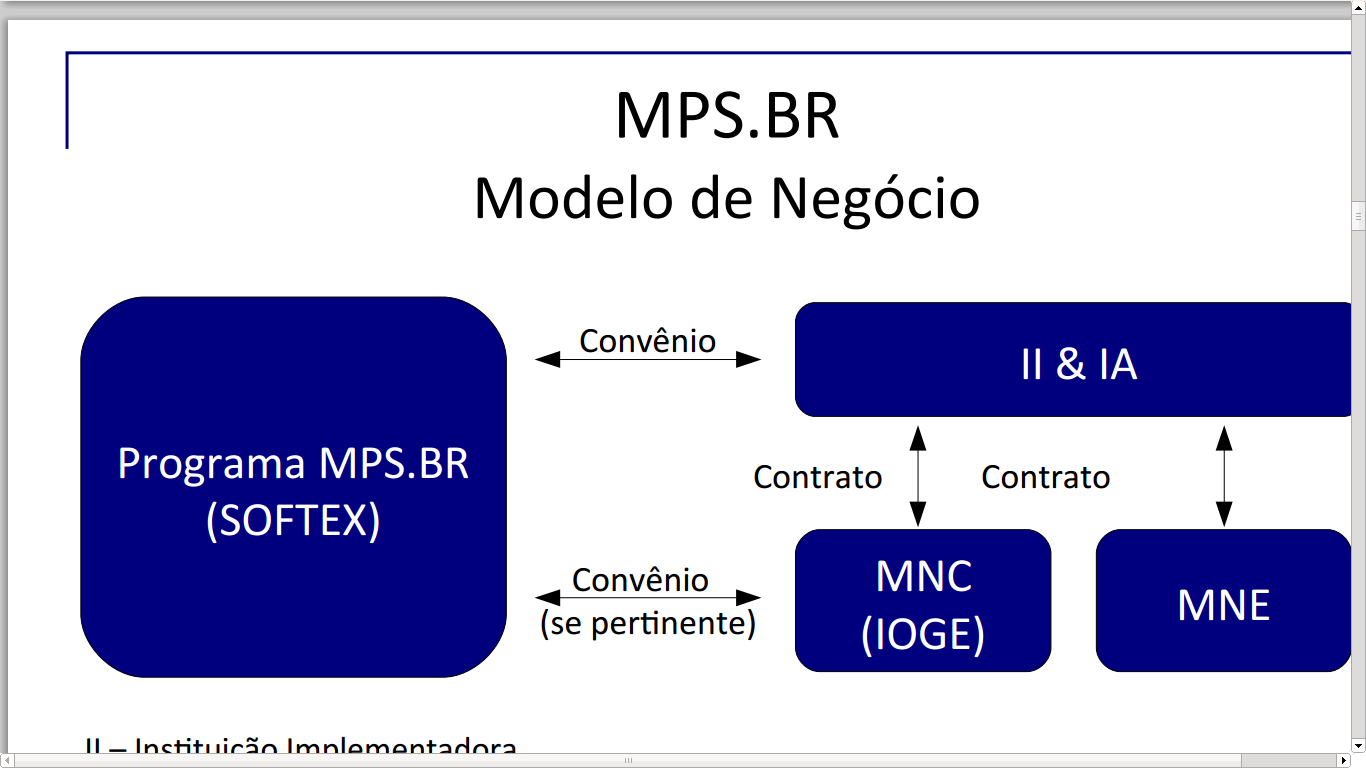
\includegraphics[scale=0.25]{MPSBR_modelo_negocios}
	\end{center}	
	\begin{enumerate}
	\item Modelo de Negócio cooperado: Várias empresas reunidas com foco de redução de custos (Pacotes utilizada para solução com várias empresas)
	\item Modelo de Negócio Específico: Empresa única (Personalizado)
	\item Convênio com o MPS.BR para tentar a redução de custo 	
	\end{enumerate}

\subsubsection{Cursos e provas}
	\begin{enumerate}
	\item Curso Introdução
	\item Curso implementadores
	\item Curso Avaliadores
	\item Curso Guia de Aquisição
	\end{enumerate}		
\subsubsection{Estrutura}
	\begin{itemize}
	\item Modelo de referência
		\begin{enumerate}
		\item Guia de implementação
		\item Guia de aquisição
		\item Guia geral
		\end{enumerate}				
		
	\item Método de Avaliação
		\begin{itemize}		
		\item Guia de Avaliação
		\end{itemize}				

	\item Método de Negócio
		\begin{enumerate}
		\item Documento do projeto
		\end{enumerate}				
	\end{itemize}		
\subsubsection{Guias}
\paragraph{Guia de Aquisição}: Contém recomendações para a condução de compra de sofware e produtos correlatos
\paragraph{Guia de Avaliação}(passo-a-passo): Contém a descrição do processo de avaliação, os requisitos para avaliador e os requisitos para avaliação.
\paragraph{Guia Geral de Sofware} : Contém a descrição dos processos e níveis do MPS.BR e detalha o MR, seus principais componentes e as defnições comuns
\paragraph{Guia de Implementação} : Contém sugestões de implementação do modelo de referência do MPS.BR
\paragraph{Guia de Geral de Serviços} : detalha o Modelo de Referência MPS para Serviços (MR-MPS-SV) e as defnições comuns necessárias para seu entendimento e aplicação

\subsubsection{Base Técnica}
	\begin{itemize}
	\item 12207
		\begin{itemize}
		\item Categoria
			\begin{itemize}
			\item Processos
				\begin{itemize}
				\item Propósitos
				\item Saídas
				\item Atividades
					\begin{enumerate}
					\item Tarefas							
					\end{enumerate}
				\end{itemize}
			\end{itemize}
		\end{itemize}			
	\end{itemize}

	\begin{itemize}
	\item CMMI
		\begin{itemize}
		\item Níveis
			\begin{itemize}
			\item Processo
				\begin{itemize}
				\item Objetivos
				\item Resultados Esperados	
				\end{itemize}
			\end{itemize}
		\end{itemize}
			
	\end{itemize}

	\paragraph{15504}(Meta-modelo)

\subsection{Guia geral} \date{31 de Março de 2014}

\subsubsection{Objetivo} Descrever de forma detalhada o MR-MPS e as definições comum.
\subsubsection{Público-Alvo} 
	\begin{itemize}
		\item Instituições avaliadoras(IA)
		\item Instituilçoes implementadores(II)
		\item outros interessados que queiram usar como referência
	\end{itemize} 
\subsubsection{Estrutura}

	\begin{itemize}
	\item Níveis de Maturidade: possui um conjunto de processos e capacidades de processo
		\begin{itemize}
		\item Processo: Lista de processos
			\begin{itemize}
			\item Propósito
				\begin{itemize}
				\item Resultados específico (Bem relacionados com as saidas da 12.207)
				\end{itemize}
			\item Capacidades(Veio da 15.504): Verificar a capacidade q o processo tem para atingir seu objetivo	
				\begin{itemize}
				\item Atributos \{Executado,\\ Gerenciado,\\ Definido,\\ Medido/controlado, \\Em otimização\\ \}
				\item Resultados: detalhar a capacidade que um processo pode ter.
				\end{itemize}					 
			\end{itemize}
		\end{itemize}			 
	\end{itemize}


\subsubsection{O que é processo?} conjunto de atividades interlacionadas que transforma entradas em saídas
	
\subsubsection{O que é capacidade de processo} caracterização da habilidade do processo em atingir os objetivos de negócio

\subsubsection{Niveis de maturidade}
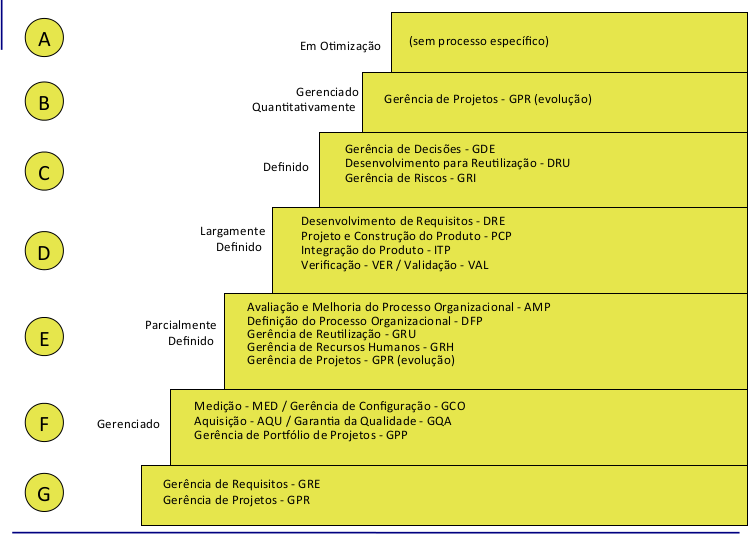
\includegraphics[scale=0.50]{niveis_maturidade}

\subsubsection{Template de definição de processos}
Nível MR-MPS.BR(maturidade)
Propósito
Resultado(s) esperado(s) \\

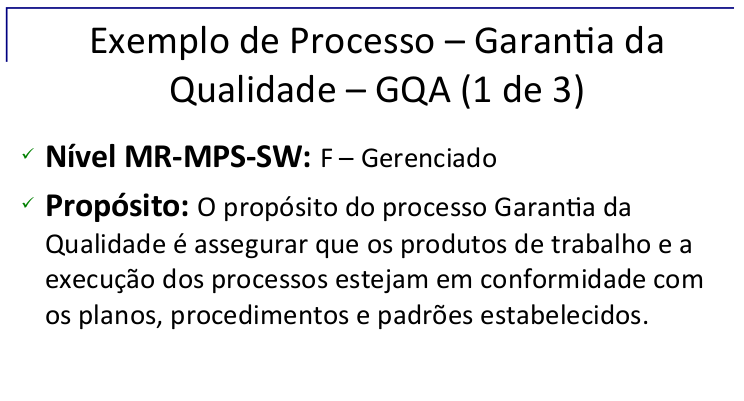
\includegraphics[scale=0.30]{exemplo_garantia_qualidade_1}
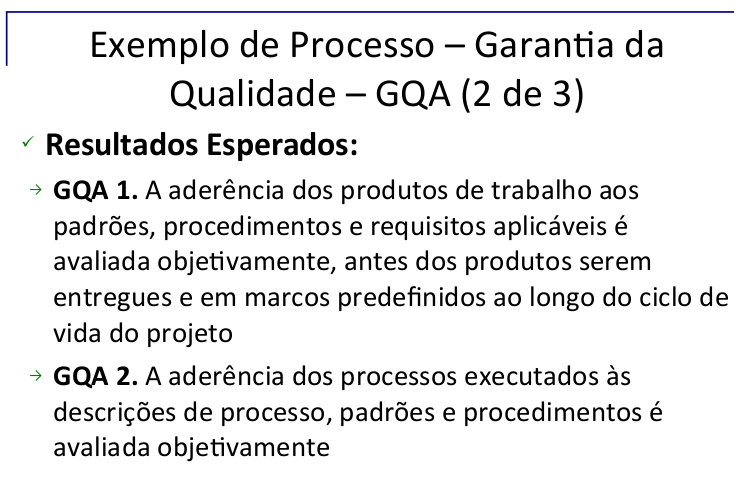
\includegraphics[scale=0.30]{exemplo_garantia_qualidade_2}
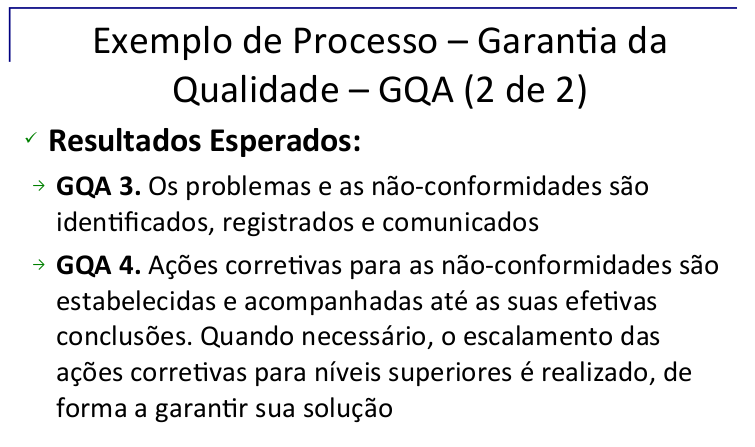
\includegraphics[scale=0.30]{exemplo_garantia_qualidade_3}


\section{CMMI para desenvolvedores} \date{2 de Abril de 2014}

\subsection{O que é SEI}
	Software Engineering INstitute \newline
	Centro de pesquisa

\subsection{O que é CMMI} 	
	Capability Maturity Model Integration \\
	Modelo de maturidade para melhoria de processo, destinado para desenvolvimento de produtos e serviços. \\
	\begin{center}
		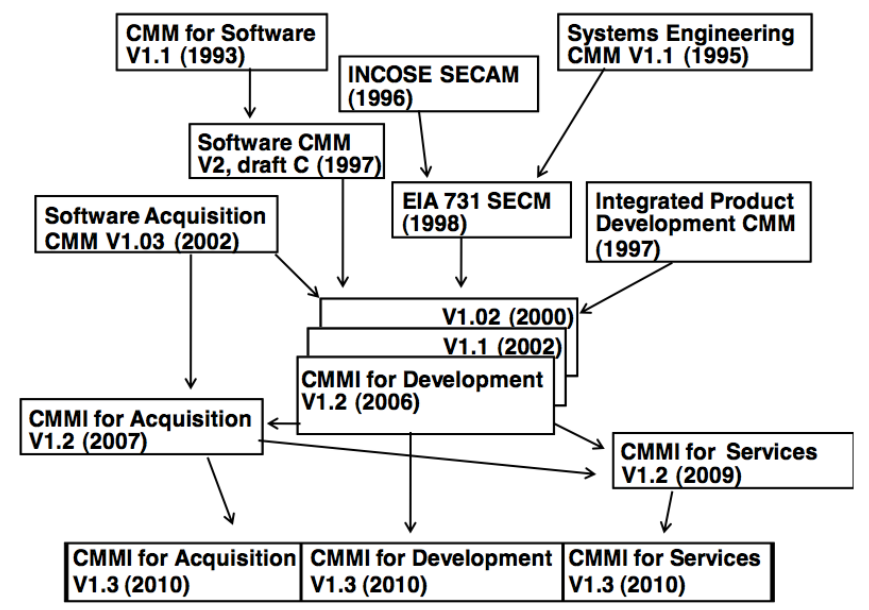
\includegraphics[scale=0.35]{historico_cmmi} \\
	\end{center}
	Foi criado para reseolver o problema originado com o uso de múltiplis CMMs.

\subsection{Conceitos}

\begin{enumerate}
\item Área de processos: Conjunto de práticas relacionadas a uma área que, quando implmentadas, satisfazem a um conjunto de metas consideradas importantes.
\item Capacidade: Habilidade do processo para alcançar ps objetivos de negócio, atuais ou futuros.
\item Maturidade: Composto por práticas específicas e genéricas relacionadas a um conjunto predefinidas de áreas de processo.
\end{enumerate}

\subsection{Como usar o CMMI}

\begin{enumerate}
\item Escolha a parte da organização alvo de melhorias.
\item Escolha um dos modelos(Development, Services ou Acquisition)
\item Escolhar uma forma de representação
	\begin{enumerate}
	\item Continua: A organização escolhe qual mprocesso melhorar
	\item Estagida (MPS usa esse!) : Formulando minha maneira de trabalhar. Escolha do mais importantea ser melhorado. Possui capacidade específica para cada nível de maturidade\\
	\begin{center}
		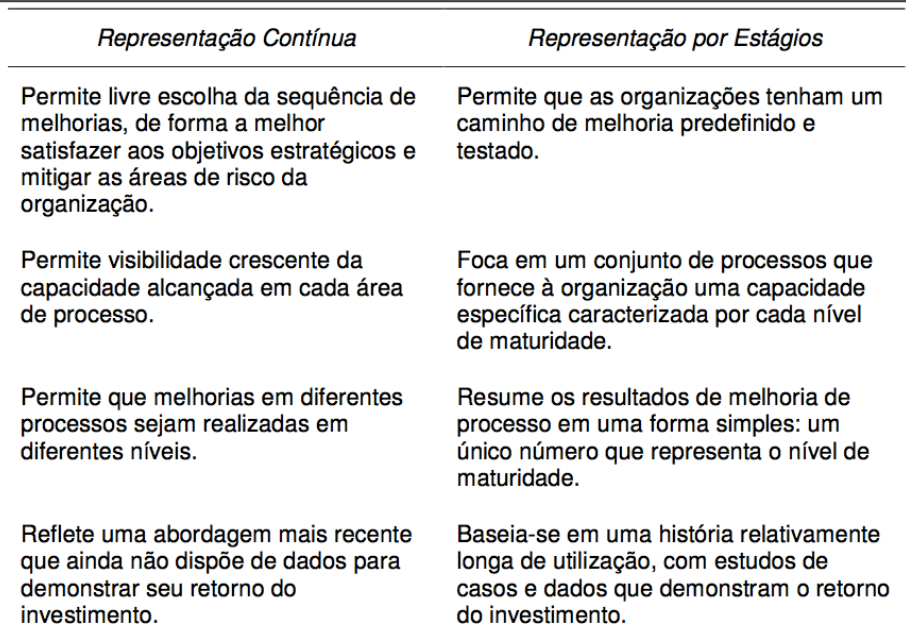
\includegraphics[scale=0.40]{representacoes_cont_estag}
	\end{center}	
	\end{enumerate}	 
\end{enumerate}	

\subsection{Estrutura de definição de Processos}
	\begin{center}
		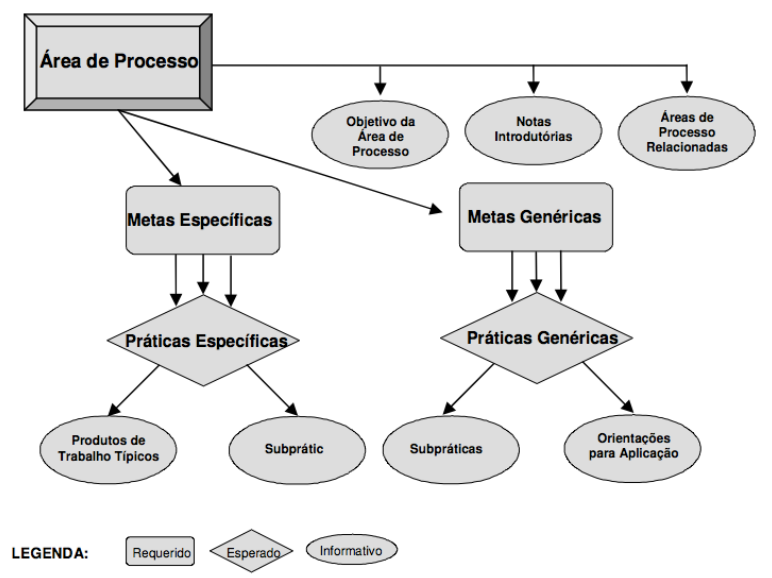
\includegraphics[scale=0.5]{estrutura_definicao_cmmi}
	\end{center}

\subsection{Categorias do precessos do CMMI para desenvolvedores}

\paragraph{Engenharia}
\paragraph{Gerenciamento de projeto}
\paragraph{Gerenciamento de processo}
\paragraph{Suporte}

\section{Métodos ágeis} \date{7 de Abril de 2014}

\subsection{Manifesto ágil}

\subsection{Scrum}
\paragraph{Dono do produto}
\paragraph{Dono do produto}
\paragraph{Dono do produto}

\subsubsection{Ciclo de vida}

\subsection{XP}
\subsubsection{Valores}
\subsubsection{Práticas XP}

\section{Avaliação de processo de software} \date{23 de Abril de 2014}

\subsection{Para que serve ?}
	\begin{itemize}
	\item Verificar o que está funcionando e o que não está
	\item Verificar aderência a um determinado modelo
	\item Definir as necessidades de melhoria de processos	
	\end{itemize}	

\subsection{Quando avaliar ?}
	ciclo IDEAL
	Avaliação no diagnóstico
	Avaliação no final do ciclo
	
\subsection{Por que avaliar?}
	Para verifivar nível de aderência a um determinado modelo de referência
	Nível de maturidade

\subsection{Como avaliar ?}
	Avaliar é medir e comparar!
	\subsubsection{Como realizar uma avaliação?}
		Depende do seu objetivo!
		Definir os objetivos de melhoria!
	\subsubsection{Como são feitas?}
		Feitas com base em algum modelo ou norma de qualidade, com o objetivo de caracterizar o processo com base no modelo.
		Os métodos existentes seguem mais ou menos os mesmos passos.
		São baseados em evidências diretas(documentação) e indiretas.
		
\subsection{Fases de um processo}
	\begin{enumerate}
	
	\item Preparar e planear avaliação
		\begin{itemize}
		\item Identificar as evidências iniciais de execução do processo
		\end{itemize}	
	\item Conduzir avaliação
		\begin{itemize}
		\item Coletar evidências e analisar
		\end{itemize}		
	\item Relatar resultados
		\begin{itemize}
		\item Um relatório da avaliação
		\end{itemize}
	\end{enumerate}

\subsection{Exemplo de Plano de avaliação de processo}
	\begin{enumerate}
	\item Necessidades e objetivos de avaliação
	\item Escopo (Organizacional e de Processos)
	\item Estratégia de Avalaição Adotada
	\item Métricas
	\item Recursos
		\begin{itemize}
		\item Pessoas
			\begin{itemize}
			\item Avaliador
			\item Participante (Processos avaliado)
			\item Patrocinador
			\end{itemize}
		\item Materiais
		\item Infra
		\end{itemize}
	\item Cronograma
	\item Aprovação
	\item Riscos associados
	\end{enumerate}

\subsubsection{Relatório de avaliação}

	\begin{enumerate}
	\item Introdução
		\begin{itemize}
		\item Como foi conduzida(estratégia)
		\item Dificuldades
		\end{itemize}
	\item Resultados
		\begin{enumerate}
		\item Processo 1
			\begin{itemize}
			\item Pontos fracos
			\item Pontos fortes
			\end{itemize}
		\item Processo 2
		\item Processo n
		\end{enumerate}
	\item Solução proposta
	\item Considerações Finais
	\end{enumerate}

\section{15504 - Método de avaliação e capacidade de processo } \date{28 de Abril de 2014}

\subsection{Objetivos}
	Determinar a capacidade dos processos de uma empresa
	Orientar a empresa para uma melhoria contínua de seus processos
	É uma norma que ajuda na criação e definição de como avaliar os níveis de capacidade
	
	Obs: Scampi e MA-MPS.BR provieram da 15504
	
\subsection{Benefícios}
	Para industrias de software
		Fornecedores 
		Organizações de desenvolvimento
	Para os compradores de software	
		Avaliar riscos da seleção de um forncedor sobre outro

\subsection{Utilização da norma}

	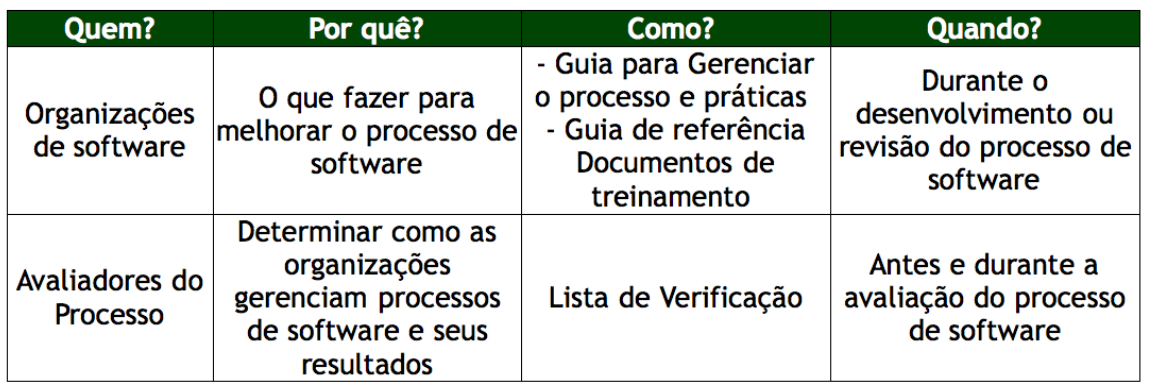
\includegraphics[scale=0.25]{utilizacao_norma}
\subsection{Composição da Norma}

	Dividida em 10 partes. 
	Foco na parte 2 e 3

\subsection{Avaliação de melhora de processos de software}

	Contexto de utilização da norma: iniciativa de melhoria de processos de software
	
	Avaliação do processo diretamente relacionada
	
	\subsubsection{Ciclo de melhoria}
	\begin{center}
		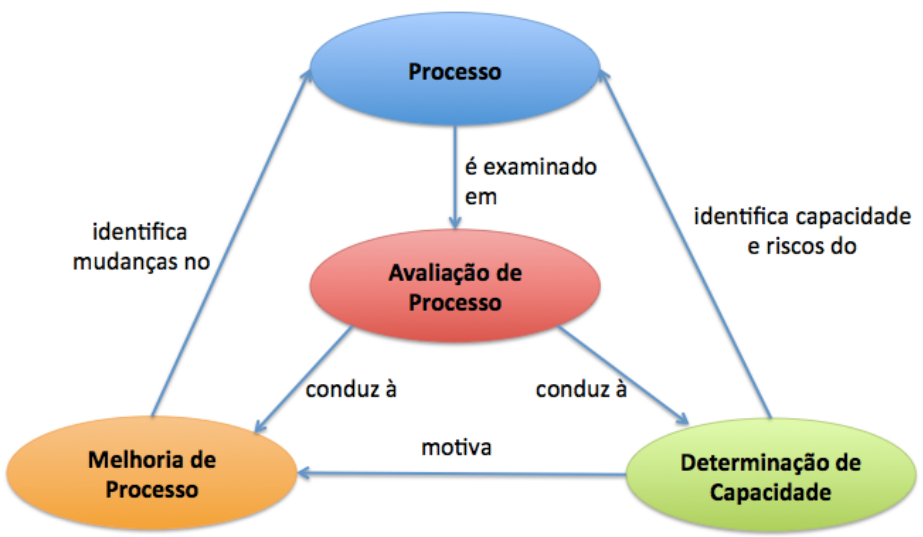
\includegraphics[scale=0.30]{ciclo_melhoria}	
	\end{center}			
		
\subsection{Parte 2 - Capacidade de processo}
	Define o conceito de capacidade de processo que é utiliado para se medir os processos avaliados

	\begin{center}
		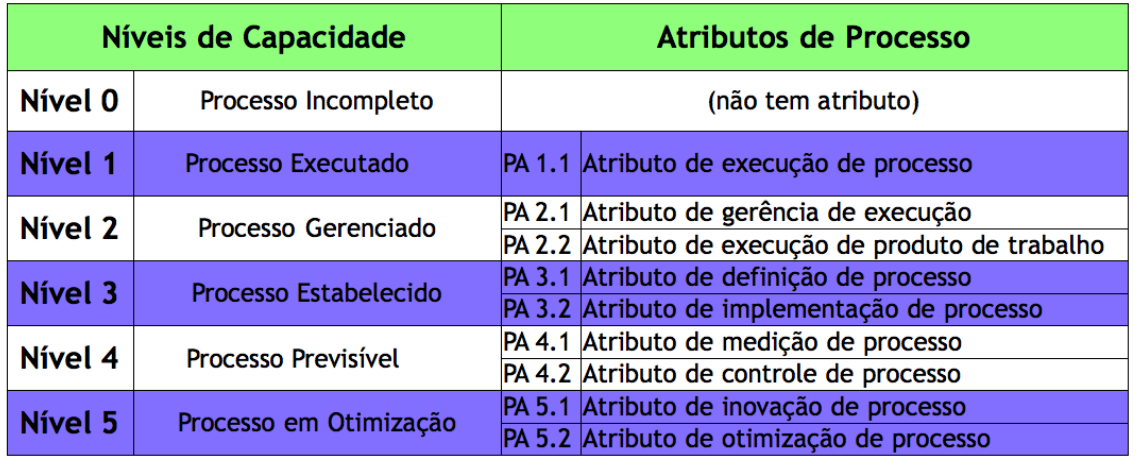
\includegraphics[scale=0.30]{capacidade_processo}
	\end{center}
	
\subsection{Níveis de capacidade}
	\subsubsection{Nível 0}
		\begin{itemize}
		\item Existe uma falha geral na satisfação do propósito do projeto
		\item Existem poucos produtos de trabalho ou resultados de processos
		
		\end{itemize}				
		
	\subsubsection{Nível 1}
		\begin{itemize}
		

		\item Propósito é alcançado, talvez de uma forma não planejada e acompanhada
		\item As pessaos da organização reconhecem quando uma ação deve eser executada e quandoo isto deve ser feito
		\item Existem produtos de trabalho evidenciando a satisfação do propósito do processo		
		\end{itemize}		

	\subsubsection{Nível 2}
		\begin{itemize}
		\item Processo planejados e acompanhados
		\item Os produtos estão conforme os padrões e requisitos especificados
		\item O processo passa a contruir produtos específicos do processo
		\item A execução do processo geram produtos de trabalho satisafazendo os requisitos de qualidade especificados, dentro do cronograma e dos recursos necessários.
		
		\end{itemize}
		
		Obs: Definição de processo e produto
	\subsubsection{Nível 3}
		\begin{itemize}
		\item Processo é executado e gerenciado
		\item O processo utiliza um processo padrão
		
		\end{itemize}
	
	\subsubsection{Nível 4}
		\begin{itemize}
		\item Processo já definido está sendo controlado.
		\item Medições detalhadas de desempenho são coletadas e analisadas
		\item A qualidade do produto é conhecida de forma quantitativa
		
		\end{itemize}
	
	\subsubsection{Nível 5}
		\begin{itemize}
		\item O desempenho do processo é continuamente melhorado
		\item O processo consegue repetibilidade em atingir suas metas de negócio definidas.	
		\item Otimizações contínuas do processo que envolve ideias novas
		
		\end{itemize}				
	
\subsection{Pontuação para determinação do Nível de Capacidade}

	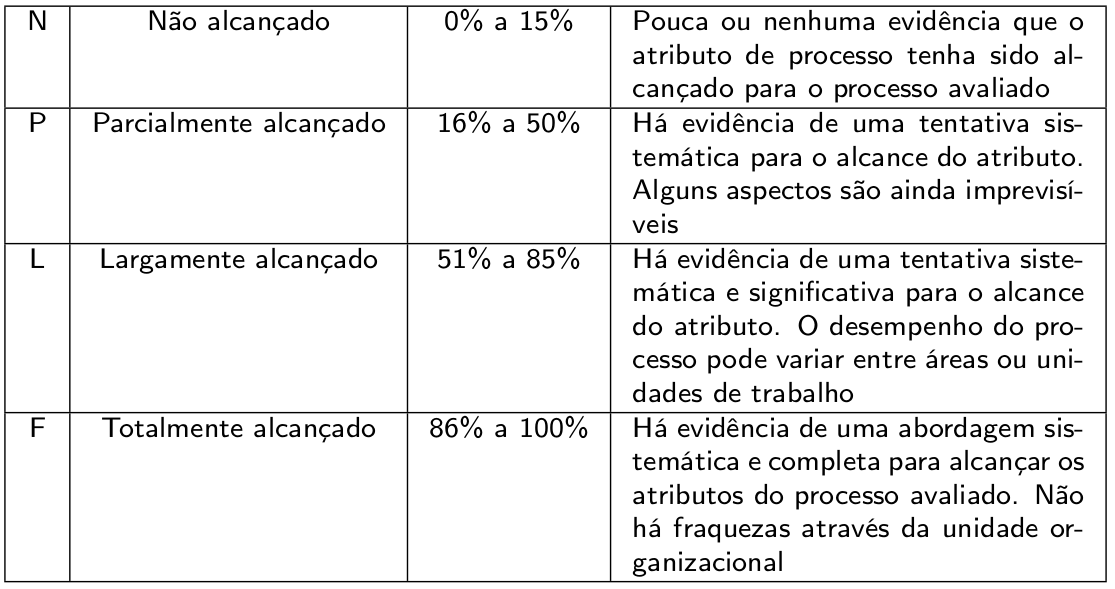
\includegraphics[scale=0.35]{tabela_pontuacao}
	
	A pontuação é acumulativa para cada nível.
	Caso tenha nivel F e L, então o nível pode ser atualmente caracterizado
	
	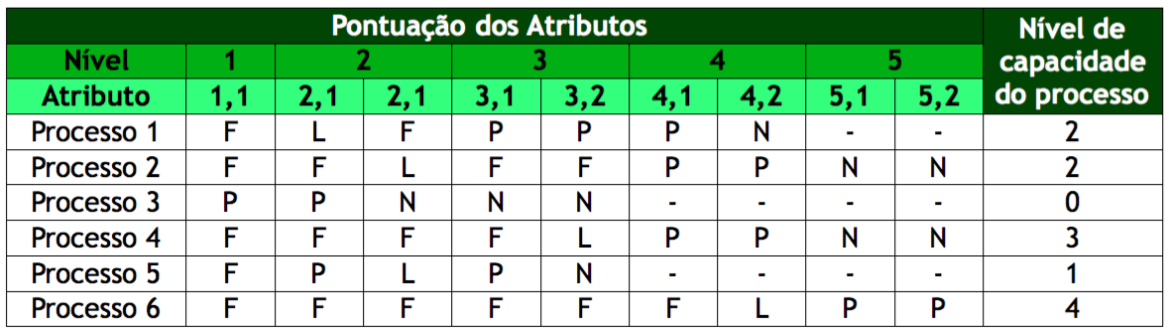
\includegraphics[scale=0.37]{exemplo_pontuacao}
\subsection{Evidências}

	\begin{itemize}
	\item Evidências diretas: Representam os resultados da implementação de uma diretiva. Exemplos de evidência direta, são planos de projeto, matriz de rastreabilidade, casos de teste.
	\item Evidências indiretas: Representam consequências indiretas da implementação da diretiva, que indicam que seus objetivos podem ser alcançados. Exemplos: templates, documentos de controle de horas, relatórios, guias.
	\item Evidências declarativas: Representam declarações coletadas através de entevistas com os integrantes do escopo organizacional avaliado, que corroboram a implementação das diretivas.
	\end{itemize}

\section{Métodos de Implementação} \date{19/05/2014}
\subsection{PDCA (Muito ligado a resolução de problemas)}
\paragraph{Usado para resolução de problemas de forma geral}
	\begin{itemize}
	\item Plan
		\begin{itemize}
		\item Identificar o problema
		\item Observar problema
		\item Analisar problema
		\item Planejar ação	
		
		\item Perguntas inclusas
			\begin{enumerate}
			\item O que eu quero melhorar?
			\item Por que eu quero melhorar?
			
			\end{enumerate}
		\item artefatos a serem gerados
			\begin{itemize}
			\item Lista de Objetivos/Problemas
			\item Plano de solução{Solução, Cronograma, Risco}
			\end{itemize}									
		\end{itemize}				

	\item Do -> Agir
		\begin{itemize}
		\item Poderia ter um artefato de: Relatório de Acompanhamento de Projeto
		\end{itemize}
	\item Check -> Verificar efetividade da solução
		\begin{itemize}
		\item Poderia ter um artefato de: Relatório de Análise da solução
		\end{itemize}
	\item Act(institucionalizar a solução)
		\begin{itemize}
		\item Padronizar solução para o problema
		\item Concluir
		\item Artefatos
			\begin{itemize}
			\item Plano de transferência da Solução
			\end{itemize}
		\end{itemize}			
		
	\end{itemize}
	
	
	\paragraph{Exercício} 
	\begin{enumerate}
	\item A forma de condução do projeto está adequada?
		\begin{itemize}
		\item Não. 
		\item Em relação ao cronograma: Houve atraso.
		\item Em relação aos objetivos da iteração 1: As definições completas eram definições. Foi parcialmente implementado por ser um processo de natureza difente
		\item Conseguiu completar as 3 primeiras partes do ciclo PDCA. Deixando a última parte para a próxima iteração.
		\end{itemize}			
	\item Objetivos estão claros?
		Está subjetivo.
	
	\item R: Não. O objetivo não foi atingido na iteração 1, isso é mostrado nas ações que estão sendo realizadas novamente nos objetivos da segunda iteração. Mostrados no objetivo 4. Mudar as ações pode ser melhor. O escopo para os objetivos pode ser menor, pois a iteração anterior não foi feita completamente, então a iteração atual(2) tenha que ser menor.
	
	\item R: Definir e institucionalizar.
	
	\end{enumerate}		


\subsection{IDEAL}
\paragraph{• Não fala como se faz a melhoria}
\paragraph{• Não propõem medição}


	\begin{itemize}
	\item Iniciaação
	\item Diagnóstico
	\item Planejamento(Estabelecimento)
	\item Ação
	\item Aprendizado(Leaveraging)
	\begin{center}
	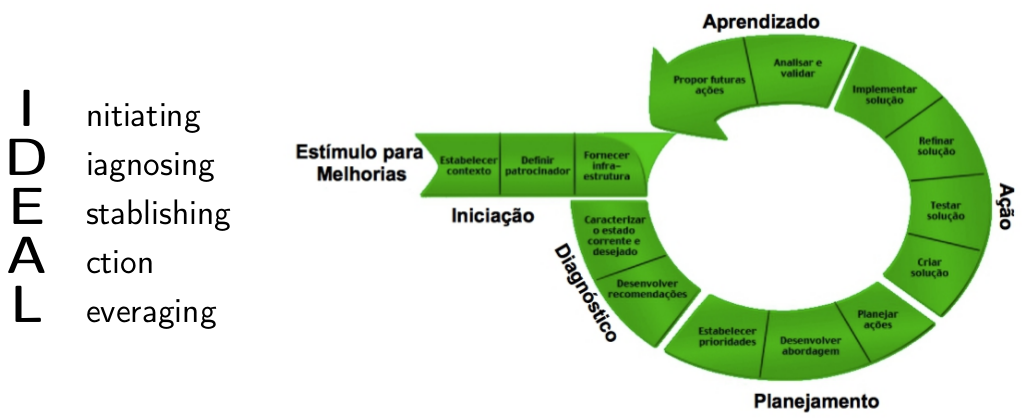
\includegraphics[scale=0.4]{IDEAL}	
	\end{center}
	
	\end{itemize}

\subsubsection{Introdução}
	Baseado em experiências do SEI
\subsubsection{Principais papéis}
	\begin{itemize}
	\item Grupo de gerência Sênior (Patrocinador)	
		\begin{itemize}
		\item Atua principalmente na fase de iniciação e planejamento
		\item Grupo define os objetivos e define o alinhamento com estes objetivos(comparado a um patrocinador) - "Quais são os objetivos?"
		\item Alocação de recursos: humanos, materiais e financeiros (Patrocínio)
		\item Monitoramento do projeto		
		\end{itemize}				
		
	\item Grupo de Processos de software
		\begin{itemize}
		\item Responsánvel por conduzir a melhoria. Definir o diagnóstico, grupo técnico, distribuir responsabilidades e monitorar
		\item Suporte, apoio em todas as fases
		\item Resolver problemas, Cronograma, alocar, Relação de acompanhamento com Grupo de Gerência Sênior		
		\end{itemize}				
		
	\item Grupo de Trabalho técnico
		\begin{itemize}
		\item Criam soluções para os problemas identificados, desenvolvem estratégias!
			\begin{itemize}
			\item Principalmente na fase de atuação			
			\end{itemize}						
		\item Implantar Soluções	
		\item Documentar, avaliar e melhorar os processos		
		\item Em pequenas empresas este grupo e o de Processo de software podem se fundir
		\end{itemize}				
	
	\end{itemize}

	
\subsubsection{Visão geral de cada fase}

\begin{itemize}
	\item Iniciação
		\begin{itemize}
			\begin{Large}
			\item Principal parte do projeto ao "iniciar"
			\item Importa-se com a estrutura
			\end{Large}					
		
		\item Entendimento do contexto e definição dos objetivos
		\item Obter compromentimento com os recursos (responsabilidade do grupo de processo de software)		
		\item Alinhamento do projeto de MPS com os objetivos de negócio!		
		\item Lista de atividades: Preocupação da criação da consciencia da melhoria(ativ. 4 e 5) 
		
		\item Resumo em uma frase Definição dos objetivos e alinhamentos dos objetivos organizacionais com os de melhoria	
		\item grupo de Processo de Software é criado	
		\end{itemize}				
	
	\item Diagnóstico/Propósito
		\begin{itemize}
		\item O que irei avaliar?
		\item Pontos fortes e fracos
		\item Estabelecimento da baseline(evidências) do estado atual da empresa
		\item Coleta de dados e condução de baseline(análise das evidências)
		\item Desenvolver solução
		\item Apresentar relatório		
		\item Lista de atividades: Atividade 4(Existem falsos-negativos?)
		
		\end{itemize}				
			
	\item Planejamento
		\begin{itemize}
		\item Definir um plano de ação
		\item Os problemas da organização são definidos		
		\item Preocupação com os esforços de melhoria existentes/medidos
		\item Lista de atividades: Atividade 7 - Identificar qualquer tipo de tentativa de melhoria
		\item Grupo de trabalho técnico é formado
		\end{itemize}
			
	\item Ação
		\begin{itemize}
		\item Desenvolver uma solução
			\begin{itemize}
			\item Testar solução - Teste em projetos piloto
			\item Implantar solução na organização - Institucionalização dos processos
			\end{itemize}
		
		\end{itemize}
			
	\item Aprendizado
		\begin{itemize}
		\item O q deu e não deu certo, se é necessário fazer outro ciclo
		\item O que é necessaŕio refinar ou não
		\item Lista de atividades		
		\end{itemize}

\end{itemize}

\subsubsection{IDEAL x PDCA}
		
\paragraph{	IDEAL = Aplicação para MPS do PDCA}		

Plan = Iniciação, Diagnóstico e Estabelecimento
Do = Ação
Check = Ação
Act = Ação e Aprendizado


\subsection{QIP} \date{28/05/2014}
\\ Editado \date{25/08/14}
\paragraph{• Consegue fazer a medição ao final do ciclo}

\subsubsection{Introdução}

\paragraph{• Possui 6 etapas}
Comparação IDEAL
	\begin{itemize}
	\item Caracterização = Iniciação e diagnóstico(IDEAL)
	\item Definir Objetivos = Iniciação e Estabelecimento
	
	\end{itemize}

\subsubsection{Fases}
\paragraph{Caracterizar}

	\begin{itemize}
	\item Identificar os problemas
	\item Diagnosticar situação atual
	
	\end{itemize}
\paragraph{Definir os objetivos}

	\begin{itemize}
	\item Definir os objetivos de melhoria
	\item Definir métricas
	\item Aplicar GQM - Derivado dos problemas da fase anterior
	\item Garantir alinhamento obejtivos de melhoria com objetivos de negócio	
	\end{itemize}
\paragraph{Escolher Processos}

	\begin{itemize}
	\item Selecionar preocessos
	\item Pensamentos em soluções
	\item Desenvolver solução
	\item Exemplo
		\begin{itemize}
		\item Falta de visibilidade das atividades - Processo: Gerência de projeto/ falta de comunicação
		\end{itemize}
	\end{itemize}
\paragraph{Executar Processos}

	\begin{itemize}	
	\item Testar a solução desenvolvida em projetos piloto
	\item Coleta de dados em relação as métricas definidas
	\item Verifica se os objetivos foram atingidos ou não
	\end{itemize}
\paragraph{Análise de dados}

	\begin{itemize}
	\item Analise de dados coletados
	\item Reavaliar as práticas atuais
	\item Gerar recomendações para projetos futuros
	\item Quais são os problemas na solução	
	\end{itemize}
\paragraph{Empacotar experiências}

	\begin{itemize}
	\item Finalizar experiência por meio da coleta de lições aprendidas e armazenamento das soluções criadas
	\end{itemize}
	
	
\subsubsection{GQM}

	\begin{itemize}
	\item Método de definição de métricas
	\item Medir Software, projeto, ...
	\item Métricas devem ser derivadas da necessidades 
	\end{itemize}	
	
	(Imagem slide 10 - Aula 23)
	
\paragraph{Fases}
	\subparagraph{Planejamento}
	\subparagraph{definição}			
	\subparagraph{Interpretação}			
	\subparagraph{Coleta de dados}			

\subsubsection{QIP x PDCA}

	\begin{enumerate}
	\item caracterização = Plan
	\item Definir objetivos = Plan
	\item Escolher processos = Plan
	\item Executar processos = Do
	\item Analiasar dados = Check
	\item Empacotar xp = Act
	\end{enumerate}


\subsubsection{QIP x IDEAL}

	\begin{enumerate}
	\item caracterização = Iniciação(ligação fraca) e Diagnóstico
	\item Definir objetivos = Iniciação/Planejamento
	\item Escolher processos = Planejamento
	\item Executar processos = Ação
	\item Analiasar dados = Ação
	\item Empacotar xp = Aprendizado

	\end{enumerate}
\subsubsection{Exercicio}

\paragraph{Dados os objetivos de melhoria abaixo, criar questões e métricas para medir o alcance deles} 
\paragraph{Aplicar GQM, fase definição de objetivos}
\begin{enumerate}
\item Objetivo:Reduzir o tempo gasto com manutenções corretivas
\item Questões:
	\begin{enumerate}
	\item Quanto tempo é gasto com Manutenções corretivas?
		\begin{enumerate}
		\item Métrica: Tempo médio gasto com manutenções corretivas
		\item Métrica: Esforço gasto com manutenções corretivas
		\item Métrica: Relação entre esforço para manutenção corretiva e manutenção evolutiva
		\item {Selecionar processos que serão alvo de melhoria, fase escolher processos}
		\item Processo projeto e construção de produto

			\begin{enumerate}
			\item Desenvolver Orientado a arquitetura
			\item Refatoração
			\item Utilizar padrão de codificação e de projeto
			\item Programação em pares 
			\end{enumerate}				
		\end{enumerate}
	\item Qual a complexidade das Manutenção corretiva?
	\item Quantidade de Manutenções corretivas ?
	\item Quais módulos possuem maior quantidade de defeitos?
	\item Quantidade de requisições envolvidas com Manutenção corretiva?
		\begin{enumerate}
		\item Coleta 1: Identificar todas as requisições do mÊs
		\item Coleta 2: Classificar as requisições
		\item Coleta 3: Contar a quantidade de RMC
		\item Computação dos dados: n - onde 'n' é a quantidade de RMC ao mês
		\item Interpretação: Quanto menor n melhor
		\item ações: Melhorar processo de teste
		\end{enumerate}
	\end{enumerate}

\end{enumerate}

	\begin{enumerate}
	\item Objetivo: Difundir o conhecimento dos sistemas pela equipe
	\item Questões
		\begin{enumerate}
		\item Quantos sistemas de difundir conhecimento?
			\begin{enumerate}
			\item Quantidade média de sistema que necessitam de treinamento
				\begin{itemize}
				\item Coleta de dados
				\item computação de dados, (somatorio Px)/n, onde Px - quantidade de sistemas com respostas < 5
				\item Responsável: GPS, definir papel caso não exista
				\item Peridiocidade: bimestralmente
				\item Interpretação: Quanto menor X, melhor
				\end{itemize}
			\end{enumerate}
		\item Acessibilidade das informações?
		\item Como está a documentação do sistema?
		\item Existem iniciativas p/ transmitir conhecimentos?		
		\end{enumerate}
	\item Ações
		\begin{enumerate}
		\item Consolidar base de conhecimentos
		\item Criar processo de consolidação do sistema
		\item Criação de processo para transferência de conhecimento(Treinamentos)
		\end{enumerate}
	\end{enumerate}
	
	\begin{enumerate}
	\item Objetivo: Melhorar a forma de distribuição de tarefas pela equipe
	\item Questões
		\begin{enumerate}
		\item Quais papeis possuem maior quantidade de tarefas?
		
		\end{enumerate}
	\end{enumerate}
\end{document}
